
\subsection{Kalibrierung der Balldetection}
\label{sec:kalibr-der-balld}
Die Ballerkennung muss zunächst kalibriert werden, da ansonsten
die ermittelte Entfernung zum Ball nicht korrekt ist. Dies ist deshalb nötig,
da die Ausrichtung der auf dem Roboter montierten Webcam
entscheidenden Einfluss auf die von der Ballerkennung ermittelten
Werte hat. Zur VisualStudio Solution ,,TP2010/11'' gehört auch ein
Unterprojekt calib. Nach Erstellung der ausführbaren Datei calib.exe
ist diese an folgende Stelle des Projektbaums zu kopieren:
\verb|\client\src\calibrate\| \\ 
Für die folgenden Schritte werden dann ein Schachbrett sowie ein
Maßband oder Ähnliches benötigt. 
Danach geht man folgendermaßen vor:
\begin{itemize}
\item Man stellt das Schachbrett und den Roboter in einen Abstand von
  ca 1 Meter voneinander entfernt so auf, dass die Kamera auf die
  Mitte des Schachbrettes zeigt. 
% TODO: bild einfügen
\item Danach misst man mit dem Maßband die Entfernung zwischen Roboter
  und Schachbrett, sowie den Abstand vom Schachbrett zum Boden (im
  Normallfall 25 cm). Die
  beiden Enden der Entfernungstrecke zeigt folgendes Bild:
 \begin{nofloat}{figure}\centering
    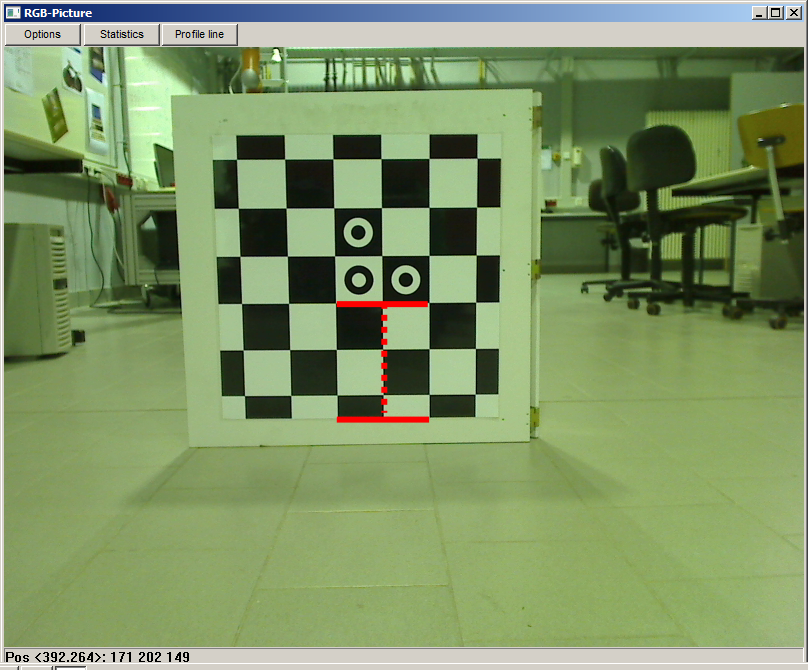
\includegraphics[width=0.55\linewidth]{bilder/camToGround_red}
    \caption{Abstand zwischen Boden und Schachbrett}
  \end{nofloat}
%TODO: bild einfügen
\item Anschließend startet man die Batchdatei \verb|calibrate.cmd| im
  Ordner \verb|\client\src\calibrate\|. Die Batchdatei fragt nun die
  Kameranummer, sowie die im vorherigen Schritt ermittelten 
 Entfernungen in mm ab und startet anschließend durch Drücken der
 Enter-Taste die Erkennung:
 \begin{nofloat}{figure}\centering
    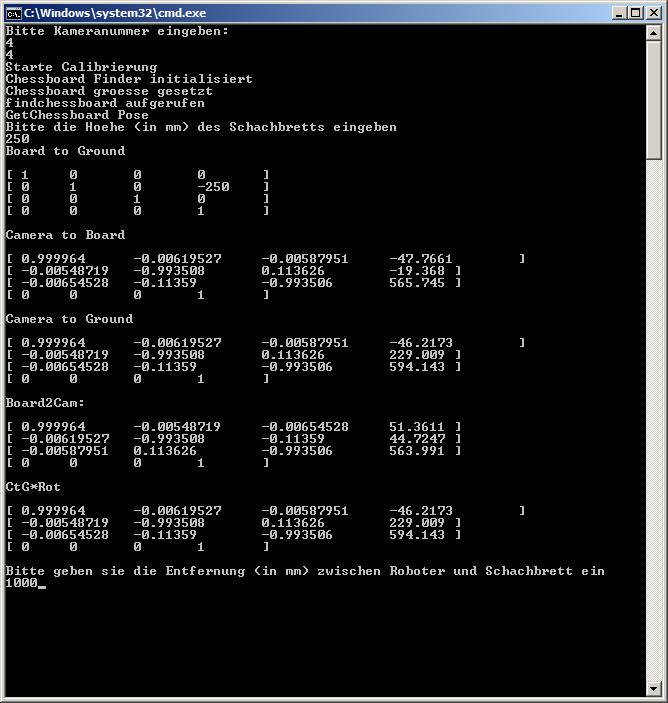
\includegraphics[width=1\linewidth]{bilder/calibrate1}
    \caption{Abfrage der zur Kalibrierung nötigen Parameter}
  \end{nofloat}\newpage
\item Die Kalibrierung ist erfolgreich, wenn folgendes Muster im
  Kamerabild angezeigt wird:
  \begin{nofloat}{figure}\centering
    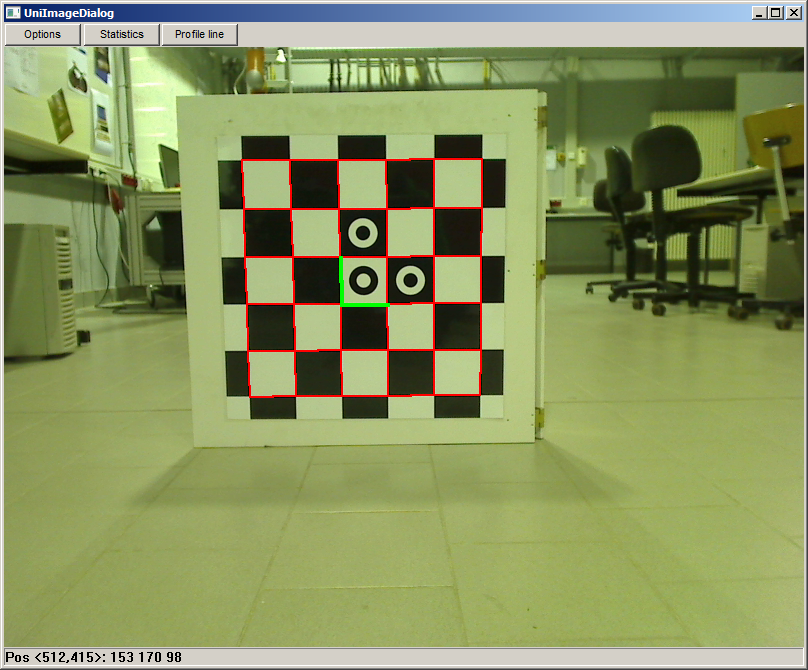
\includegraphics[width=0.7\linewidth]{bilder/calibrate2}
    \caption{Darstellung einer erfolgreichen Kalibrierung der Ballerkennung}
  \end{nofloat}
\item Dann ist im Batch-Skript die Ausführung
  des Kalibiertools mit \textless STRG \textgreater -C zu unterbrechen. Auf die Nachfrage,
  ob auch die Batchdatei unterbrochen werden soll, gibt man ,,n'' ein:
 \begin{nofloat}{figure}\centering
    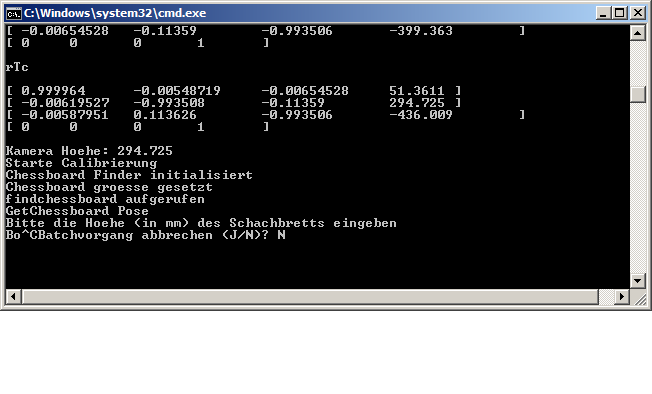
\includegraphics[width=\linewidth]{bilder/calibrate3}
  \end{nofloat}\newpage
\item Danach sollte ein neuer Ordner im aktuellen Verzeichnis mit den
  Kalibrierdaten sein. Er hat als Bezeichnung die Kameranummer
  erhalten. Im folgenden Bild sieht man das Ergebnis einer
  erfolgreichen Kalibrierung für die Kamera mit der Nummer 4, es wurde
  ein neues Verzeichnis \verb|cam4| mit den Kalibrierungsdateien erzeugt:
 \begin{nofloat}{figure}\centering
    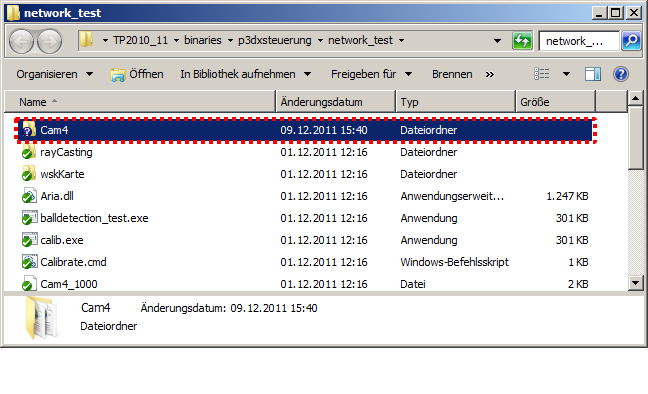
\includegraphics[width=\linewidth]{bilder/calibrate4_red}
  \end{nofloat}
\end{itemize}
%%% Local Variables: 
%%% mode: latex
%%% TeX-master: "template"
%%% End: 
